\section{Introduction}

Speech emotion understanding has long been framed as a classification problem. Early systems relied on hand-crafted acoustic features \cite{elayadi2011survey, ververidis2006emotional}; subsequent advances in deep learning introduced end-to-end architectures that learn discriminative representations directly from audio \cite{trigeorgis2016adieu}. Self-supervised learning (SSL) further transformed the landscape, enabling models such as wav2vec~2.0 \cite{Wav2vec2}, HuBERT \cite{HuBERT}, and WavLM \cite{WavLM} to acquire powerful speech representations from large unlabeled corpora. More recently, specialized models such as \textit{emotion2vec} \cite{emotion2vec} have introduced distillation frameworks explicitly targeting universal emotion representations, achieving robust benchmark performance. Despite these advances, all such approaches share a fundamental constraint: they map rich, continuous human affect into a fixed set of discrete labels \cite{SUPERB}, losing the nuance carried by breathiness, vocal tension, sarcasm, and dynamic tonal shifts. Consider two calls to a customer service center: one from a caller who is angry but maintains controlled, clipped articulation, and one from a caller who is distressed and confused, with fragmented speech and rising intonation at every phrase boundary. A categorical SER system maps both to \textit{angry}; yet the appropriate downstream response—immediate escalation to a supervisor versus patient clarifying dialogue—differs entirely. This gap is not incidental: it reflects a fundamental mismatch between the discrete output space of categorical SER and the continuous, multi-dimensional nature of human affective expression in real conversation.

The emergence of speech language models (SLMs) offers a promising alternative by reframing emotion inference as open-ended auditory reasoning. Foundational models such as SALMONN \cite{SALMONN} and Qwen-Audio \cite{Qwen-Audio} established an encoder-connector-LLM architecture, enabling free-form text descriptions of affective states. Scale expansions have since pushed the boundaries further: Step-Audio~2 \cite{Step-Audio2} incorporates a latent audio encoder for fine-grained paralinguistic recognition, Kimi-Audio \cite{Kimi-Audio} employs extensive flow-matching pre-training, and MOSS-Audio \cite{MOSS-Audio} introduces time-marker insertion to preserve temporal prosody. Yet without explicit emotion specialization, these general-purpose SLMs remain prone to acoustic grounding failures and paralinguistic hallucinations---generating affective narratives not fully supported by the audio signal \cite{Qwen2-Audio}. \Cref{tab:paradigm_comparison} contrasts these paradigms.

\begin{table}[ht]
\centering
\footnotesize
\setlength{\tabcolsep}{5pt}
\renewcommand{\arraystretch}{1.2}
\begin{tabular}{@{}>{\raggedright\arraybackslash}p{0.24\linewidth}>{\raggedright\arraybackslash}p{0.26\linewidth}>{\raggedright\arraybackslash}p{0.40\linewidth}@{}}
\toprule
\textbf{Paradigm} & \textbf{Output} & \textbf{Positioning} \\
\midrule
Categorical SER & Closed-set emotion label & Efficient for classification, but limited in fine-grained paralinguistic description. \\
General-purpose audio MLLMs & Prompted label or description & Flexible across audio tasks, but not emotion-specialized. \\
Amphion EmoAnalyzer & SER label + DEA narrative & Bilingual emotion-specialized model with DEA-focused Emotional DPO. \\
\bottomrule
\end{tabular}
\caption{Comparison of speech emotion understanding paradigms. DEA denotes descriptive emotion analysis.}
\label{tab:paradigm_comparison}
\end{table}

% TODO: convert to TikZ figure (domain-constraints.mdc §9)
\begin{figure}[ht]
\centering
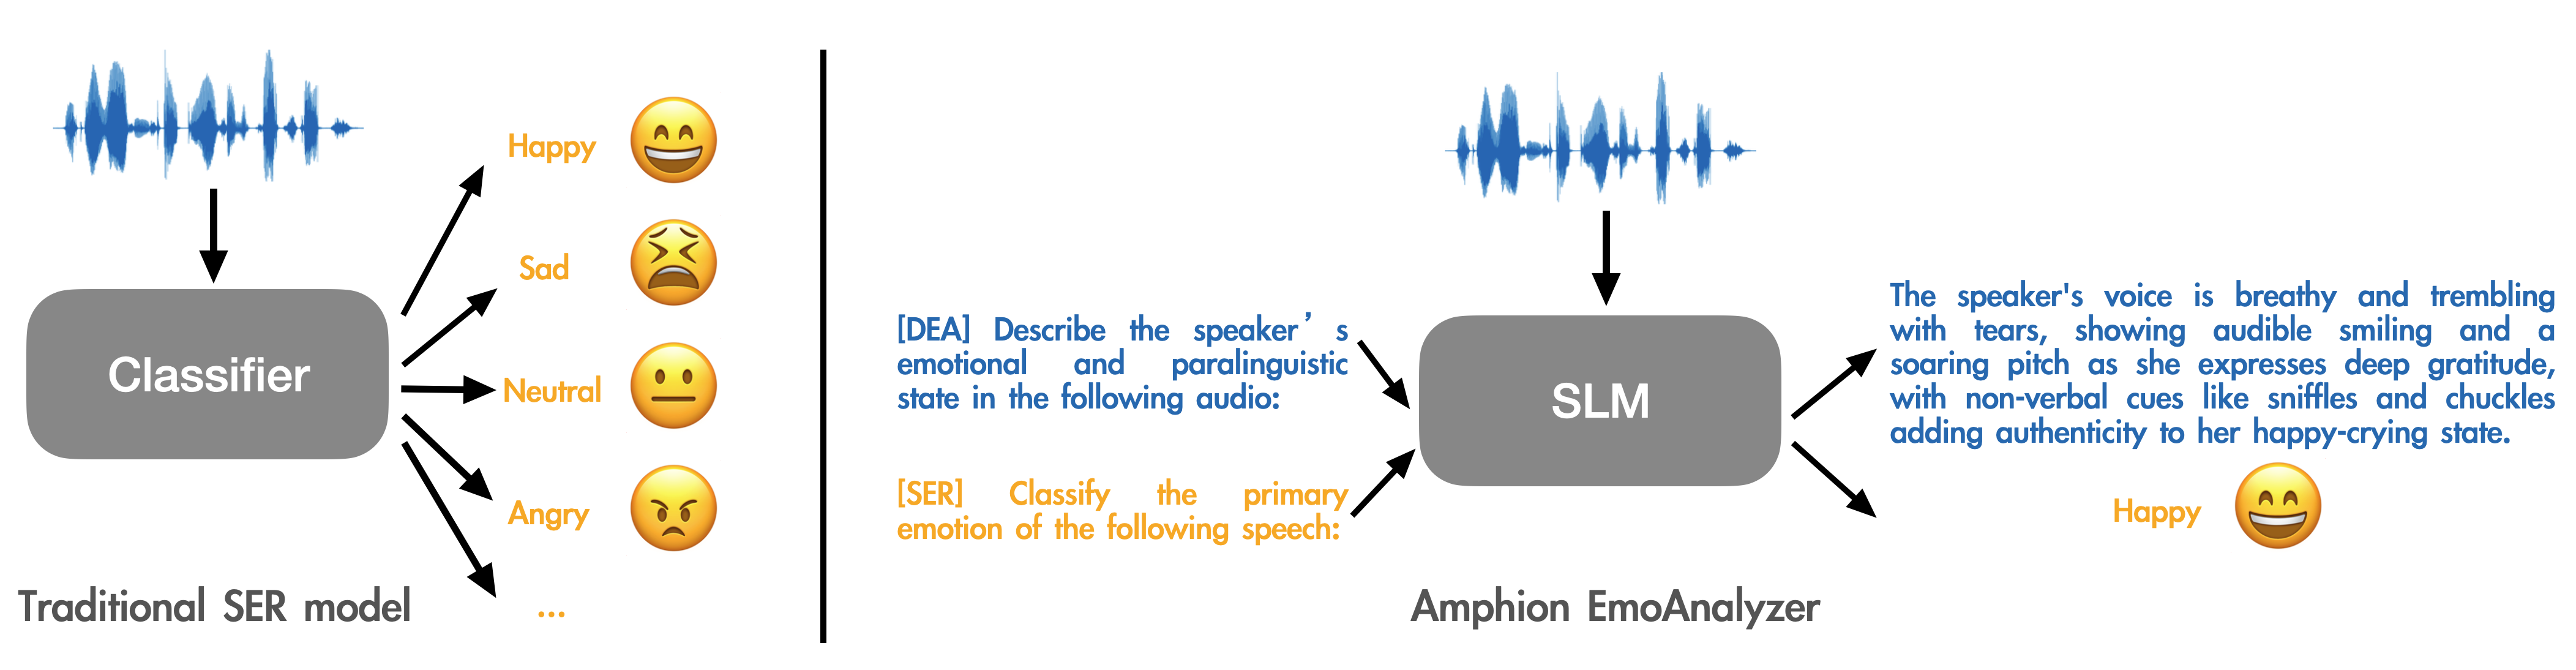
\includegraphics[width=\linewidth]{images/multi_task_ser_v2.png}
\caption{Comparison between traditional categorical SER and our proposed descriptive emotion analysis (DEA) task flow. Instead of mapping audio to a rigid, closed-set emotion category, DEA generates fine-grained, natural-language narratives detailing the speaker's emotional state and paralinguistic cues.}
\label{fig:task_schematic}
\end{figure}

To bridge this gap, we introduce \textbf{Amphion EmoAnalyzer}, a compact bilingual speech emotion understanding model that jointly supports \textit{speech emotion recognition} (SER) and \textit{descriptive emotion analysis} (DEA). EmoAnalyzer is designed to reason over both what is said and how it is spoken: ASR grounds the model in semantic content, SER provides reliable categorical emotion recognition, and DEA generates natural-language descriptions of the speaker's emotional state and paralinguistic cues.

Two ingredients make this capability practical for real-world speech. First, we developed a structured data curation pipeline that uses frontier MLLMs to extract multi-dimensional vocal profiles, followed by human-in-the-loop adjudication guided by an expert SER model \cite{emotion2vec}. This pipeline produced a high-confidence bilingual proprietary dataset encompassing over 1,000 hours of conversational speech. Second, we introduce Emotional Direct Preference Optimization (Emotional DPO), a DEA-focused alignment strategy that improves descriptive fidelity on difficult cases such as sarcasm, tonal shifts, and acoustic degradation.

Our primary contributions are summarized as follows:
\begin{itemize}
    \item \textbf{Comprehensive Multi-task Modeling:} We present Amphion EmoAnalyzer, an efficient 1.5B-parameter model for joint categorical SER and natural-language DEA.
    \item \textbf{Emotional DPO for DEA:} We introduce a domain-specific alignment strategy that improves descriptive emotion fidelity and mitigates paralinguistic hallucinations on complex acoustic edge cases.
    \item \textbf{High-Fidelity Data Curation Pipeline:} We develop a scalable annotation methodology combining structured MLLM profiling, expert-model verification, and human-in-the-loop adjudication to construct a curated 1,000-hour bilingual (En/Zh) proprietary corpus.
    \item \textbf{Strong SER and DEA Performance:} EmoAnalyzer achieves the best average results in our five-dataset SER benchmark (45.49\% vs.\ 37.05\% UA over the leading SLM baseline) and surpasses Gemini-3.0-Flash in descriptive emotion fidelity.
\end{itemize}

The demo page is available at \ldots, and we will release the human curated 1,000-sample test set.% TODO: add demo URL before release
